\section{Philosophy and methods}
\label{sec:philosophy_and_methods}

\subsection{Social and Aesthetic Philosophy - TBA}
\label{sec:philosophy}

\begin{mdframed}
\textbf{Key ideas: social, language, emergence, dialogue, training\ldots what else?}

Relatively mainstream philosophy: Hume, Bergson, Mead, Dewey, Bakhtin,
Gilligan, Nietzche, Sloterdijk.  Aesthetic philosophers, and poets
writing on aesthetics: Collingwood, Colleridge, Carver, Keats, Kant.
\end{mdframed}

\subsection{Methods: ``What are the proposed `lab rats'?''}
\label{sec:methods}

\begin{figure}
\resizebox{\columnwidth}{!}{%
%% For final:
\begin{tikzpicture}
%  \draw[thick] (4,0) node[below={2cm}] {\emph{A.~``mere generation''}}
%                     pic[red, -latex]{darc=100:270:1.3cm:Chicken:Lay:2.4cm:3cm}
%                     pic[red, -latex]{uarc=280:450:1.3cm:Egg:Hatch:1cm:.1cm};
%
  \draw[thick] (4.0,0) node[below={2cm},align=center] {\emph{A.~how to become a writer\footnotemark}}
                      pic[red, -latex]{darc=100:270:1.3cm:{}:{Write for 8 hours a day}:1cm:.3cm}
                      pic[red, -latex]{uarc=280:450:1.3cm:{}:{Read for 8 hours a day}:1cm:.3cm};
%
  \draw[thick](8.5,0) node[below={2cm}] {\emph{B.~``the Other''}}
                     pic[red, -latex]{darc=100:270:1.3cm:Statement:Speak:2.1cm:2.6cm}
                     pic[red, -latex]{uarc=280:450:1.3cm:Response:{Listens and interprets}:.2cm:.1cm};

%  \draw[thick] (4,-5.5) node[below={2.2cm}] {\emph{D.~learning by doing}}
%                        pic[red, -latex]{darc=100:240:1.5cm:Poet:Write:3cm:2.7cm}
%                        pic[red, -latex]{rarc=250:320:1.5cm:Poem:Responds:1cm:.5cm}
%                        pic[red, -latex]{uarc=330:450:1.5cm:Context:Speaks:1cm:.1cm};
%
%
  \draw[thick] (13,0) node[below={2cm}] {\emph{C.~proto-workshop}}
                        pic[red, -latex]{larc=100:180:1.3cm:Poet:Writes:1cm:.2cm}
                        pic[red, -latex]{rarc=190:270:1.3cm:Poem:Responds:1cm:.4cm}
                        pic[red, -latex]{rarc=280:360:1.3cm:Context:Speaks:.7cm:.7cm}
                        pic[red, -latex]{larc=370:450:1.3cm:Reader:Responds:.8cm:.2cm};

%  \draw[thick] (13,-5.5) node[below={2.2cm}] {\emph{F.~how computers work}}
%                       pic[red, -latex]{darc=100:180:1.5cm:{}:Print:1.5cm:1.4cm}
%                       pic[red, -latex]{rarc=190:270:1.5cm:{}:Loop:1cm:1.4cm}
%                       pic[red, -latex]{rarc=280:360:1.5cm:{}:Read:1cm:1.4cm}
%                       pic[red, -latex]{larc=370:450:1.5cm:{}:Eval:1.4cm:.2cm};
% Note:
% controls at end: offset of outer text, followed by offset of inner text
\end{tikzpicture}

%% For quick compiling
% 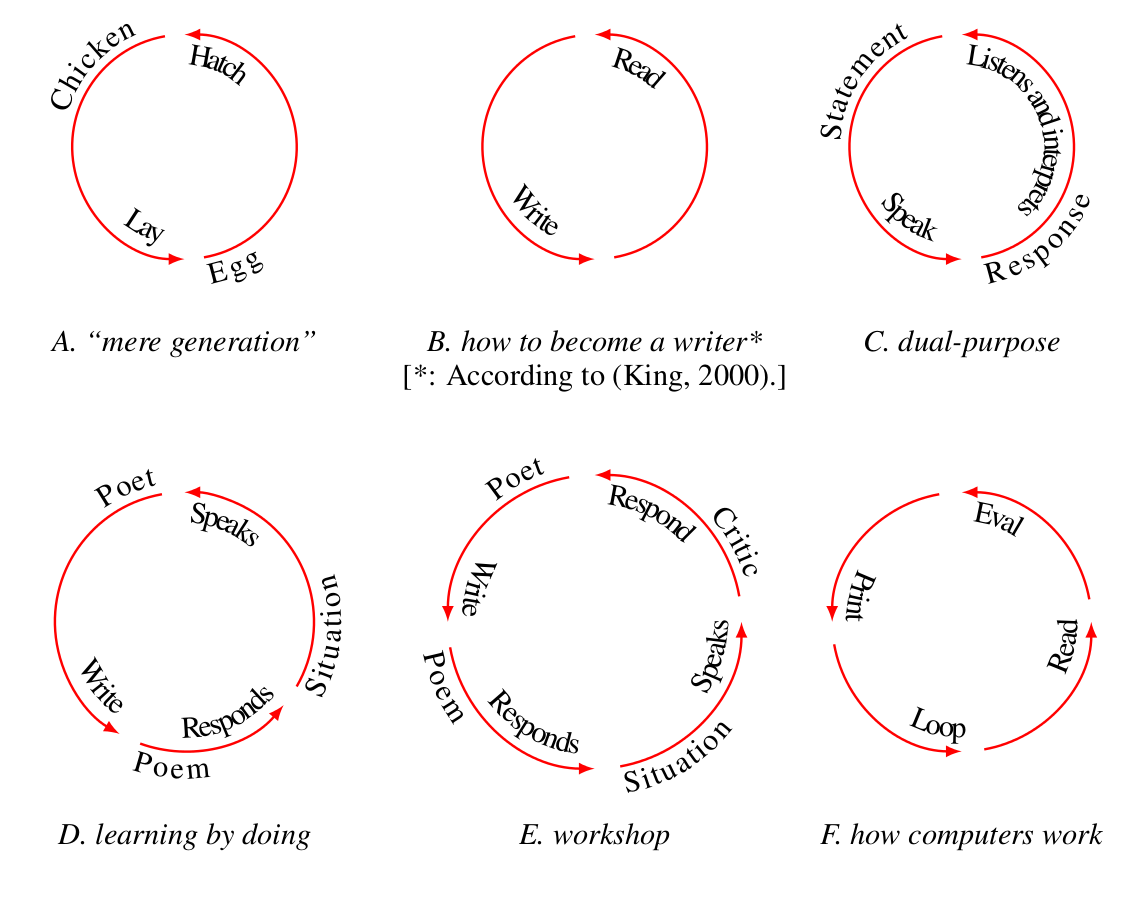
\includegraphics{figures/cycles_shortcut}
}

\caption{(A) gives a simple recipe for the growth and
development of a writer;
(B) \emph{response} always has dimensions that goes beyond the
utterance that is overheard;
(C) adds a \emph{reader} who shares the context with the writer and responds.%, and who responds to this context particularly as it is expressed through the poem
\label{fig:cycles}}
\end{figure}


There are many possible places for a ``dialogical'' intervention
within the writing process; see Figure \ref{fig:cycles}.  Figure
\ref{fig:cycles}(A) shows the standard chicken-and-egg problem, which
provokes the question of \emph{evolution}; 1(B) shows an analogous
picture that gives a simple recipe for the growth and development of a
writer; 1(C) is a formally similar diagram that squares up to the
metalinguistic features of the situation, showing that a
\emph{response} (which may be verbal, visceral, physical or something
else) always has dimensions that goes beyond the utterance that is
overheard; 1(D) examines in further detail what happens when someone
\emph{writes} -- namely, writing as a response to a situation that may
allow the writer to make sense of this situation; 1(E) adds a
\emph{critic} who responds to the situation, particularly as it is
expressed through and enhanced by the poem; 1(F) shows that this
situation is not an entirely unfamiliar for computer programmers,
especially considering that the ``Eval'' phase in a Read-Eval-Print
loop be interrupted with a debugger to fine-tune program operation.

In \cite{serendipity-arxiv}, we described a related template for a
pattern language for interactions in a computational poetry workshop:
%%
\begin{quote}
{\tt presentation}, {\tt listening}, {\tt feedback}, {\tt questions}, and
{\tt reflections}.
\end{quote}
To this should be added the potential for real-time {\tt replies} to
{\tt questions} before subsequent ``offline'' {\tt reflections}.  We
used this template to expand several of the patterns of serendipity
described by \cite{van1994anatomy}, showing how they could be used to
foster discovery and invention in a workshop environment.

Our ``lab rats'' are, accordingly, not poems -- which could, after
all, be developed through ``mere generation'' -- but are, rather,
\emph{instances of reading and responding to poetry}.  This may take
place within a formal ``workshop'' context or they may take place in
smaller-scale experiments where a computer system reads and responds
to other poets.  Naturally, such responses can also be more or less
``canned'' (as with Michael Cook's humorously nonspecific
AppreciationBot), so the question becomes what constitutes an
authentic, interesting, or useful response, and how will these be
developed?  The idea of responses is also useful at the micro-level,
as will be made clear in the following section.

%%% Local Variables: 
%%% mode: latex
%%% TeX-master: "poetryICCC"
%%% End: 
